% !TeX program = pdflatex
\documentclass[tikz,border=8pt]{standalone}
\usepackage{tikz}
\definecolor{FigureBlue}{HTML}{2563EB}\definecolor{FigureOrange}{HTML}{EA580C}
\begin{document}
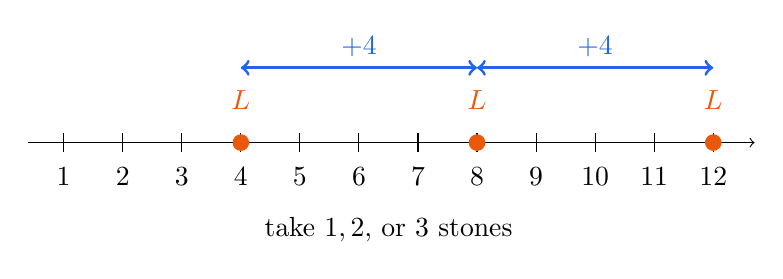
\begin{tikzpicture}[x=.75cm]
  \draw[->] (.4,0)--(12.7,0);
  \foreach \n in {1,...,12}{\draw (\n,-.12)--(\n,.12);\node[below=2mm] at (\n,0) {$\n$};}
  \foreach \n in {4,8,12}{\fill[FigureOrange] (\n,0) circle (3pt);\node[above=3mm,FigureOrange] at (\n,0) {$L$};}
  \draw[<->,FigureBlue,line width=1.1pt] (4,.95)--node[above] {$+4$}(8,.95); \draw[<->,FigureBlue,line width=1.1pt] (8,.95)--node[above] {$+4$}(12,.95);
  \node at (6.5,-1.1) {take $1,2,$ or $3$ stones};
\end{tikzpicture}
\end{document}
